       \begin{center}
            \chapter{HARDWARE AND SOFTWARE}
        \end{center}
	
	
	\begin{center}
	{\Large\textbf{\section{Apparatus}}}
	\end{center}
    For our project, We required hardware and software(Code). Both of them are important to us to build a Wireless Power Transmission System for Charging Electric Vehicles We are using Arduino UNO R3, Ultrasonic Sensors, and Relay to make our project more advanced. We also use multi-functional power like Solar Power, Battery, and Electric Power. Now we discuss each and every apparatus briefly.
	\vspace{3\baselineskip}
    \subsection{Arduino UNO R3} 
	 The Arduino Uno board can be built with power pins, analog pins, ATmegs328, ICSP header, reset button, power LED, digital pins, test LED 13, TX/RX pins, USB interface, an external power supply. The Arduino UNO board description is discussed below.
	

	\begin{figure}[H]
	\centering
	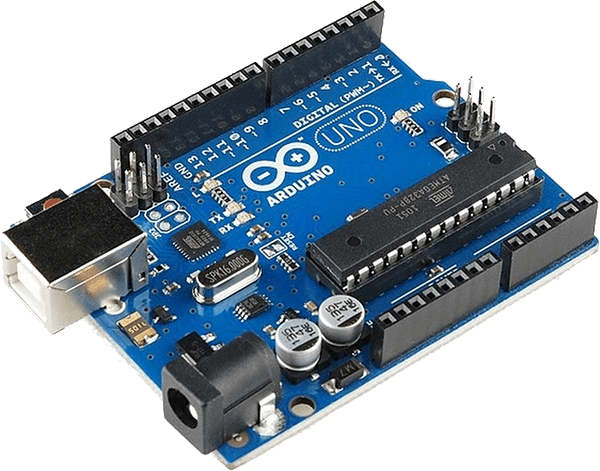
\includegraphics[width=10.75cm,height=8.44cm]{./images/image2.png}
        \caption{Arduino Uno R3}
	\end{figure}
	
	
	
	
	\vspace{3\baselineskip}
	\begin{itemize}
		\item \textbf{Power Supply}
	
	\end{itemize}
    The Arduino Uno power supply can be done with the help of a USB cable or an external power supply. The external power supplies mainly include AC to DC adapter otherwise a battery. The adapter can be connected to the Arduino Uno by plugging into the power jack of the Arduino board. Similarly, the battery leads can be connected to the Vin pin and the GND pin of the POWER connector. The suggested voltage range will be 7 volts to 12 volts.

       

	
	
	\begin{itemize}
        \item  \textbf{Input \&\ Output}
	
	The 14 digital pins on the Arduino Uno can be used as input $\&$ output with the help of the functions like pinMode(), digitalWrite(), $\&$ Digital Read().
	
	\vspace{1\baselineskip}
	\textbf{Pin1 (TX) $\&$ Pin0 (RX) (Serial):} This pin is used to transmit $\&$ receive TTL serial data, and these are connected to the ATmega8U2 USB to TTL Serial chip equivalent pins.

 

	
	\textbf{Pin 2 $\&$ Pin 3 (External Interrupts):}  External pins can be connected to activate an interrupt over a low-value, change in value.

        \vspace{1\baselineskip}
        \textbf{Pins 3, 5, 6, 9, 10, $\&$ 11 (PWM):} This pin gives 8-bit PWM o/p by the function of analogWrite(). 

        \vspace{1\baselineskip}
        \textbf{SPI Pins (Pin-10 (SS), Pin-11 (MOSI), Pin-12 (MISO), Pin-13 (SCK):}These pins maintain SPI communication, even though offered by the fundamental hardware, are not presently included within the Arduino language.

        \vspace{1\baselineskip}
        \textbf{Pin-13(LED): }The inbuilt LED can be connected to pin-13 (digital pin). As the HIGH-value pin, the light-emitting diode is activated, whenever the pin is LOW. 

        \vspace{1\baselineskip}
        \textbf{ Pin-4 (SDA) $\&$ Pin-5 (SCL) (I2C):} It supports TWI communication with the help of the Wire library.


        \vspace{1\baselineskip}
       \textbf{ AREF (Reference Voltage):}The reference voltage is for the analog i/ps with analogReference(). 


         \vspace{1\baselineskip}
         \textbf{ Reset Pin: }This pin is used for resetting (RST) the microcontroller

         \end{itemize}

	
	\begin{itemize}
		\item \textbf{Memory} The memory of this Atmega328 Arduino microcontroller includes flash memory-32 KB for storing code, SRAM-2 KB EEPROM-1 KB.
	
        \end{itemize}

	\begin{itemize}
		\item \textbf{Communication} \\ The Arduino Uno ATmega328 offers UART TTL-serial communication, and it is accessible on digital pins like TX (1) and RX (0). The software of an Arduino has a serial monitor that permits easy data. There are two LEDs on the board like RX $\&$ TX which will blink whenever data is being broadcasted through the USB. A Software Serial library permits serial communication on Arduino Uno digital pins and the ATmega328P supports TWI (I2C) as well as SPI communication. The Arduino software contains a wired library for simplifying the utilization of the I2C bus. 
	
	\end{itemize}

	\textbf{* The features of Arduino Uno R3 includes the following:}
	
	\begin{itemize}
		\item The operating voltage is 5V
	
		\item  The recommended input voltage will range from 7v to 12V
	
		\item  The input voltage ranges from 6v to 20V
	
		\item  Digital input/output pins are 14
	
		\item  Analog i/p pins are 6
	
		\item  DC Current for each input/output pin is 40 mA
	
		\item  DC Current for 3.3V Pin is 50 mA
	
		\item  Flash Memory is 32 KB
	
		\item  SRAM is 2 KB
	
		\item  EEPROM is 1 KB
	
		\item CLK Speed is 16 MHz
	
	\end{itemize}

	\newpage
	\subsection{LCD Display} LCDs is that when an electrical current is applied to the liquid crystal molecule, the molecule tends to untwist. This causes the angle of light that is passing through the molecule of the polarized glass and also causes a change in the angle of the top polarizing filter. As a result, a little light is allowed to pass the polarized glass through a particular area of the LCD.
	\begin{figure}[H]
	\centering
	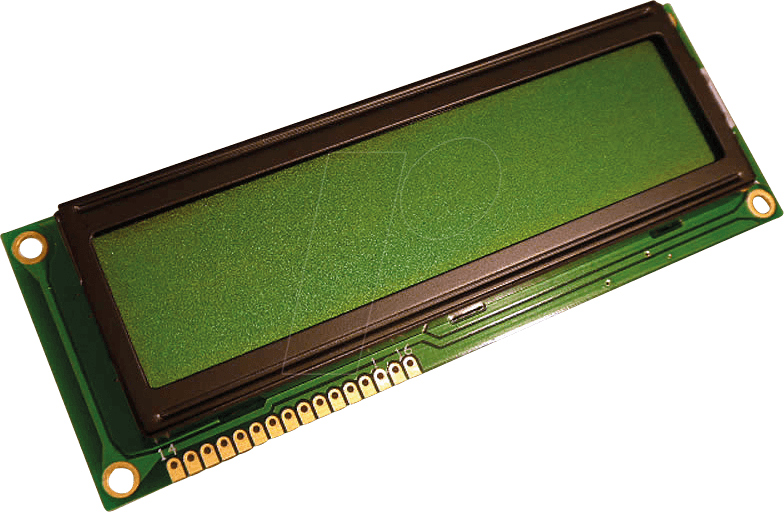
\includegraphics[width=9.86cm,height=5.62cm]{./images/image3.png}
        \caption{LCD Display}
	\label{fig:speed_is_mhz__312}
	\end{figure}
	
	

	
	
	Lorem Ipsum is simply dummy text of the printing and typesetting industry. Lorem Ipsum has been the industry's standard dummy text ever since the 1500s, when an unknown printer took a galley of type and scrambled it to make a type specimen book. It has survived not only five centuries, but also the leap into electronic typesetting, remaining essentially unchanged. It was popularised in the 1960s with the release of Letraset sheets containing Lorem Ipsum passages, and more recently with desktop publishing software like Aldus PageMaker including versions of Lorem Ipsum.
	\vspace{3\baselineskip}
    \begin{center}
        \Large Write here with your requirements.
    \end{center}
	\vspace{3\baselineskip}



\subsection{Ultrasonic Sensor} Ultrasonic sensor working principle is either similar to sonar or radar which evaluates the target/object attributes by understanding the received echoes from sound/radio waves correspondingly. These sensors produce high-frequency sound waves and analyze the echo which is received from the sensor. The sensors measure the time interval between transmitted and received echoes so that the distance to the target is known.

        \vspace{1\baselineskip}

	
	\begin{figure}[H]
	\centering
	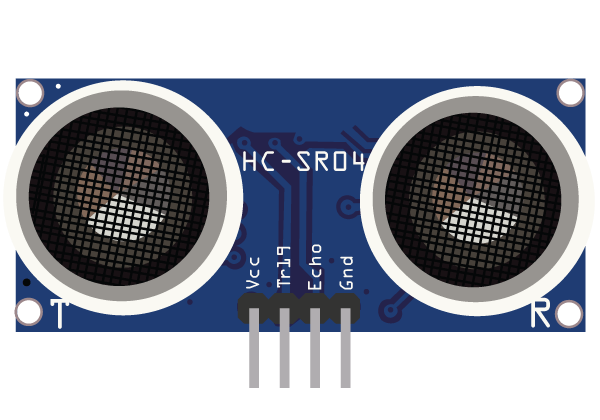
\includegraphics[width=10.89cm,height=6.64cm]{./images/image4.png}
	\caption{Ultrasonic Sensor}
	\label{fig:ultrasonic_sensor}
	\end{figure}
	
	
	
	\vspace{5\baselineskip}
	Lorem Ipsum is simply dummy text of the printing and typesetting industry. Lorem Ipsum has been the industry's standard dummy text ever since the 1500s, when an unknown printer took a galley of type and scrambled it to make a type specimen book. It has survived not only five centuries, but also the leap into electronic typesetting, remaining essentially unchanged. It was popularised in the 1960s with the release of Letraset sheets containing Lorem Ipsum passages, and more recently with desktop publishing software like Aldus PageMaker including versions of Lorem Ipsum.
	\vspace{3\baselineskip}
    \begin{center}
        \Large Write here with your requirements.
    \end{center}
	\vspace{3\baselineskip}

	
		\subsection{Relay (5 Volts)} Lorem Ipsum is simply dummy text of the printing and typesetting industry. Lorem Ipsum has been the industry's standard dummy text ever since the 1500s, when an unknown printer took a galley of type and scrambled it to make a type specimen book. It has survived not only five centuries, but also the leap into electronic typesetting, remaining essentially unchanged. It was popularised in the 1960s with the release of Letraset sheets containing Lorem Ipsum passages, and more recently with desktop publishing software like Aldus PageMaker including versions of Lorem Ipsum.
	\vspace{3\baselineskip}
    \begin{center}
        \Large Write here with your requirements.
    \end{center}
	\vspace{3\baselineskip}
	
	\begin{figure}[H]
	\centering
	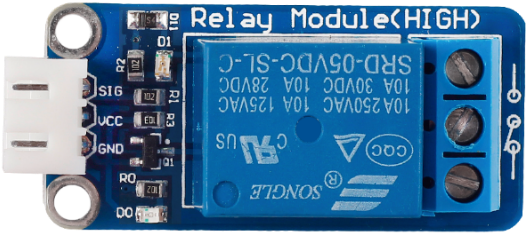
\includegraphics[width=11.59cm,height=6.16cm]{./images/image5.png}
	\caption{Relay (5 Volts)}
	\label{fig:5_volt_relay}
	\end{figure}
	
	
	\vspace{1\baselineskip}
	Solid state relays will have a sensing element to sense the input voltage and switch the output using opto-coupling.\break
	
  \textbf{* Testing of a Relay}
	

	Since they are electromechanical devices, relays can wear out eventually and stop working overtime. But there are a few techniques to test if a relay is working or not. These techniques include:
	\break
	\begin{itemize}
		\item Testing a Relay with a Multimeter
	
		\item Build a simple circuit to test the Relay
	
		\item Use a DC Power Supply to see whether a relay is functioning properly
	\end{itemize}


\subsection{Mini Tesla Coil}
Lorem Ipsum is simply dummy text of the printing and typesetting industry. Lorem Ipsum has been the industry's standard dummy text ever since the 1500s, when an unknown printer took a galley of type and scrambled it to make a type specimen book. It has survived not only five centuries, but also the leap into electronic typesetting, remaining essentially unchanged. It was popularised in the 1960s with the release of Letraset sheets containing Lorem Ipsum passages, and more recently with desktop publishing software like Aldus PageMaker including versions of Lorem Ipsum.
	\vspace{3\baselineskip}
    \begin{center}
        \Large Write here with your requirements.
    \end{center}
	\vspace{3\baselineskip}
	

	\begin{figure}[H]
	\centering
	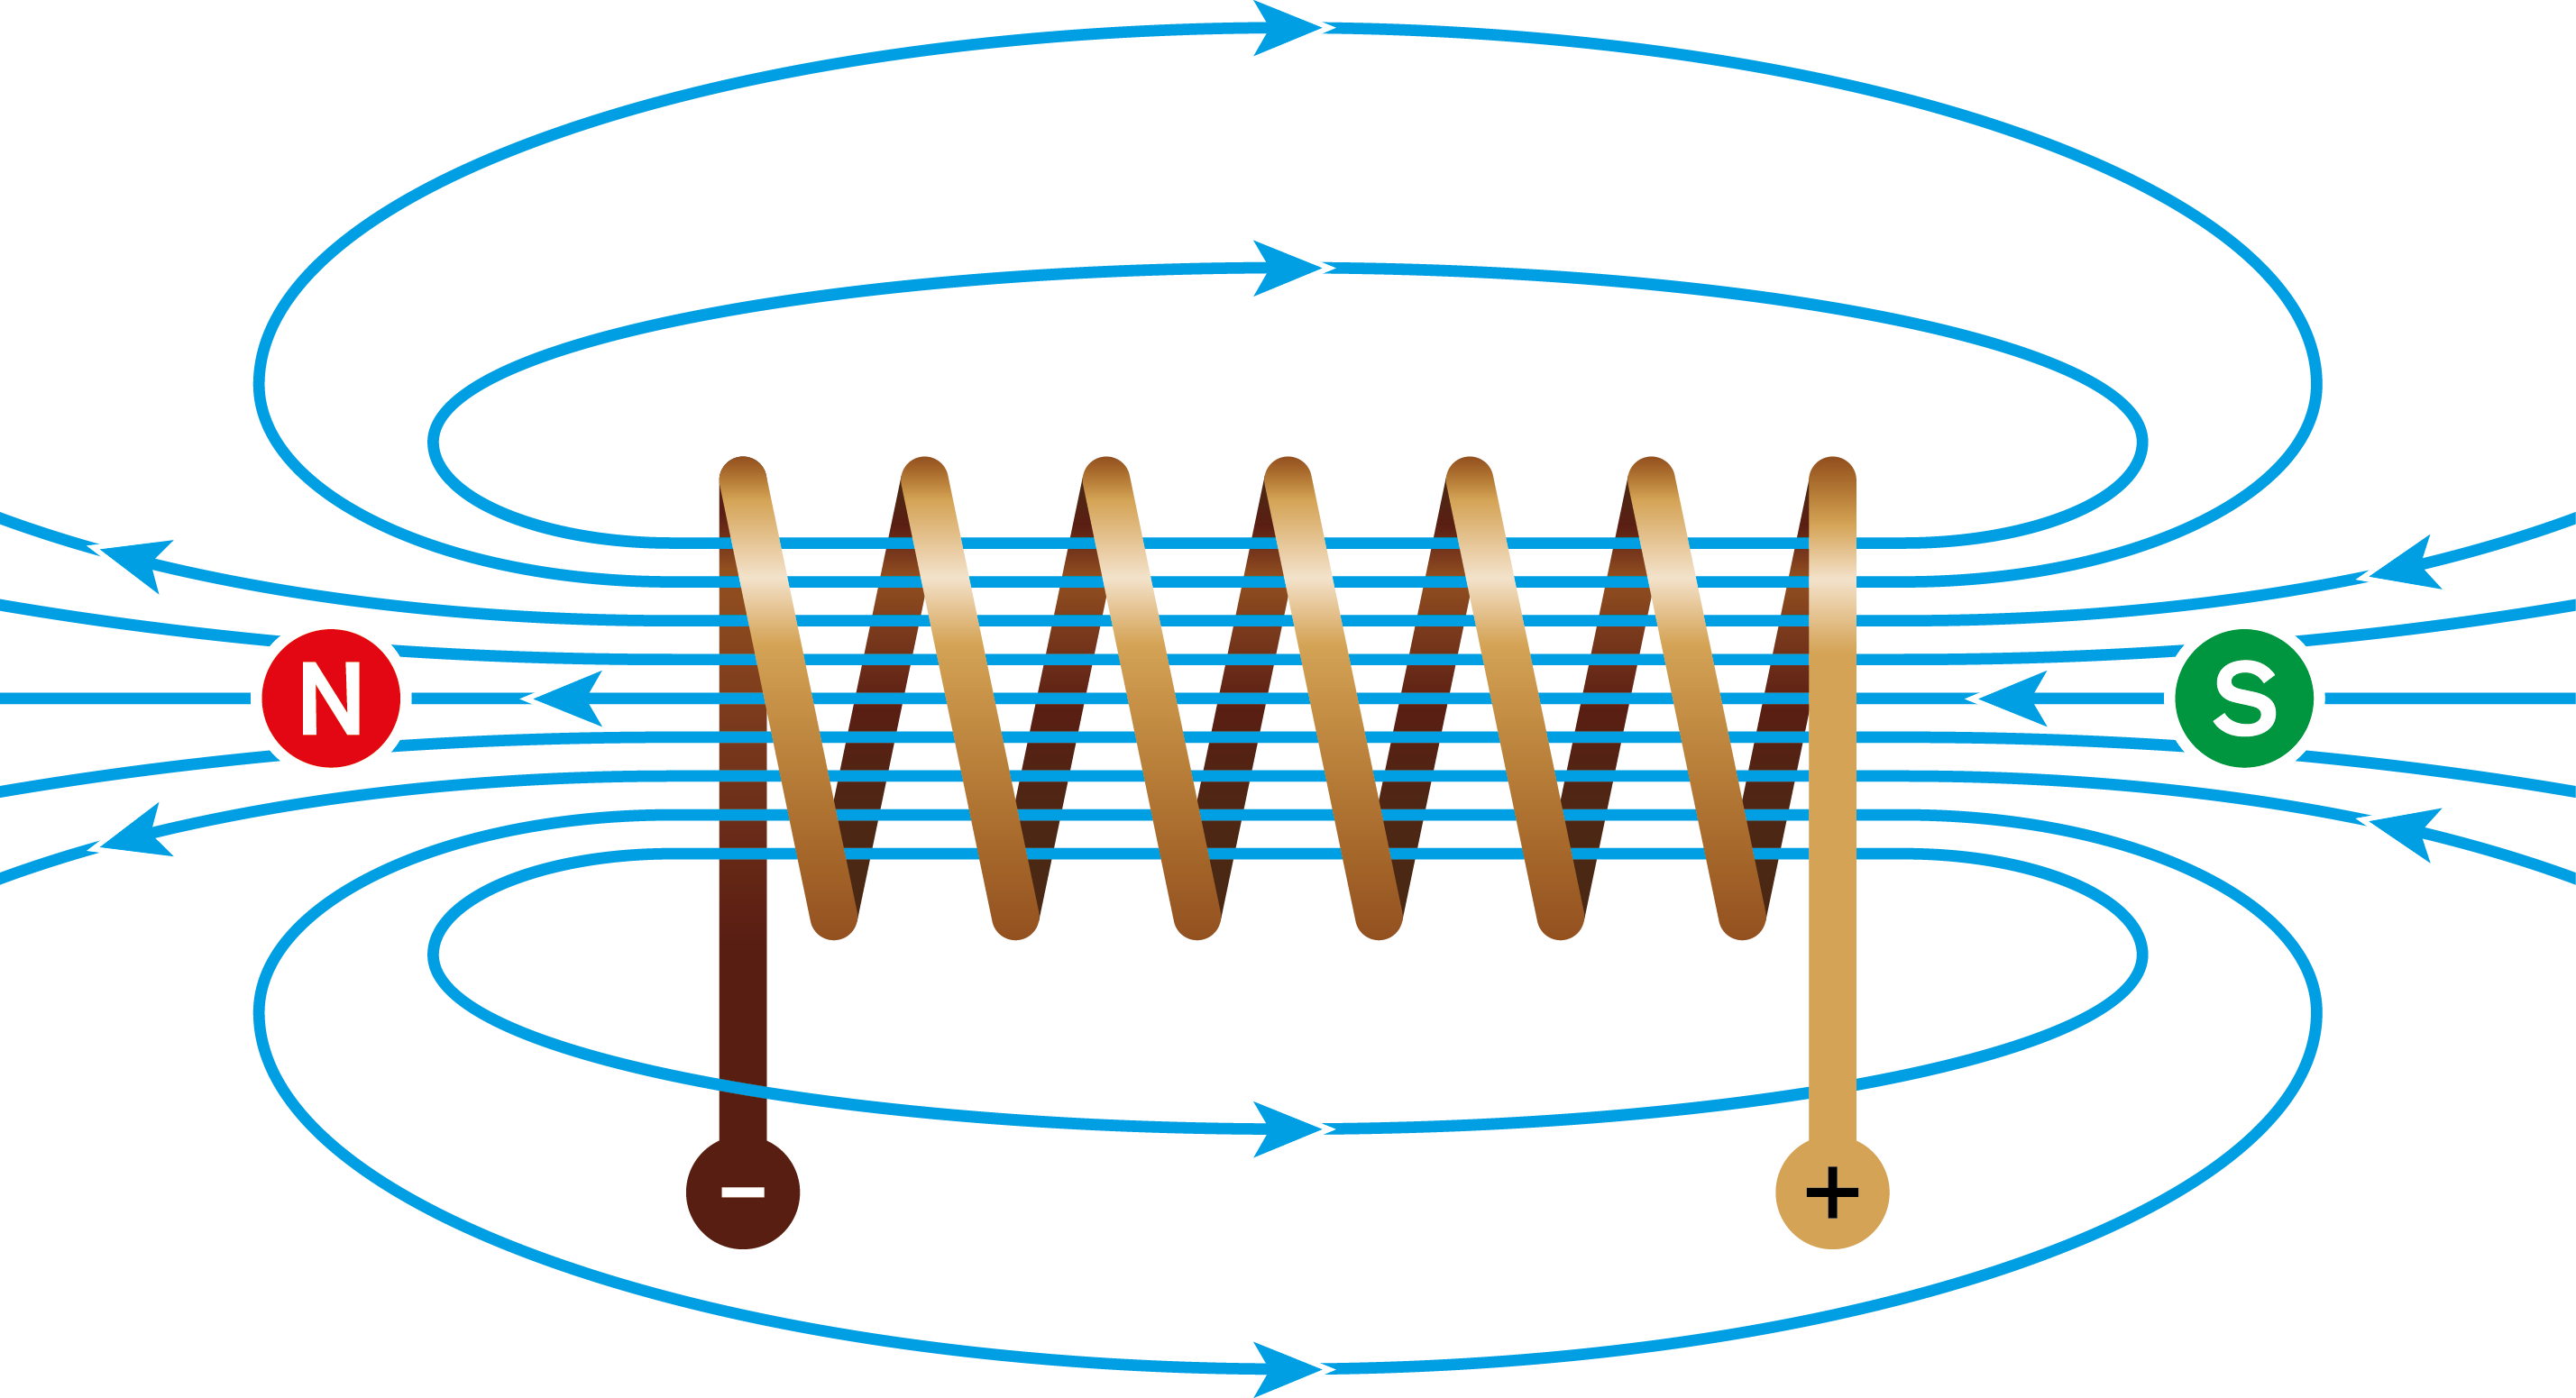
\includegraphics[width=11.14cm,height=6.05cm]{./images/image6.png}
        \caption{Tesla Coil}

	\end{figure}
	
	
	\vspace{1\baselineskip}
	
	
	
	\vspace{1\baselineskip}
	Setting up a Tesla coil with an adjustable rotary spark gap gives the operator more control over the voltage of the current it produces. This is how coils can create crazy lightning displays and can even be set up to play music timed to bursts of current.
	
	While the Tesla coil does not have much practical application anymore, Tesla’s invention completely revolutionized the way electricity was understood and used. Radios and televisions still use variations of the Tesla coil today.
	
	
	\newpage


	\subsection{Solar Panel} When the sun shines onto a solar panel, energy from the sunlight is absorbed by the PV cells in the panel. This energy creates electrical charges that move in response to an internal electrical field in the cell, causing electricity to flow.


	
	\begin{figure}[H]
	\centering
	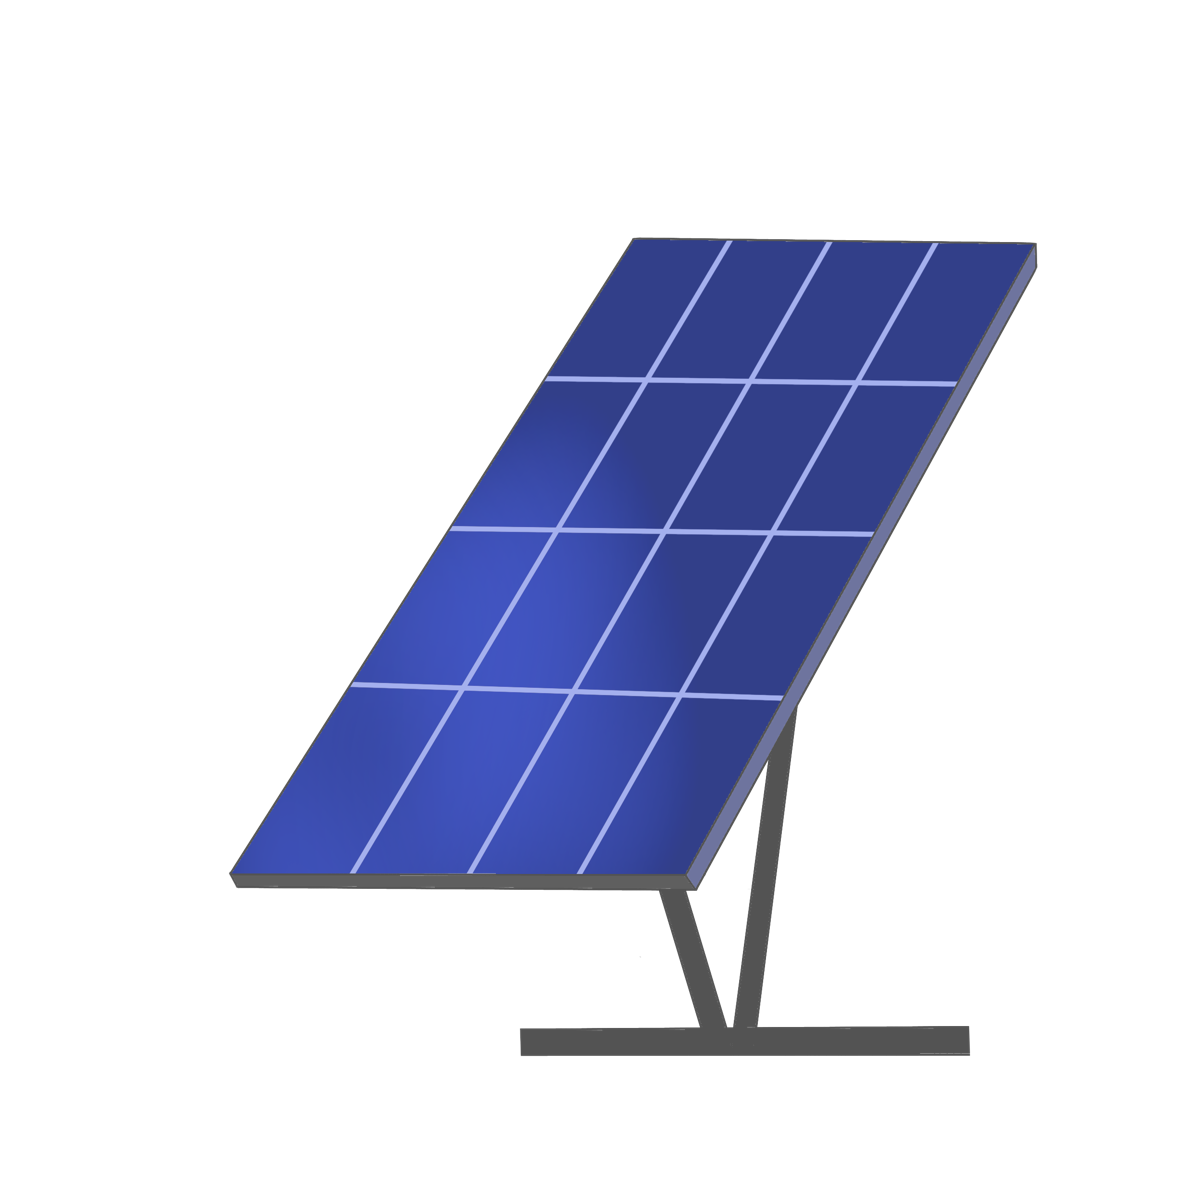
\includegraphics[width=9.17cm,height=7.83cm]{./images/image7.png}
	\caption{Solar Panel}
	\label{fig: solar_panel}
	\end{figure}
	
	
	\vspace{1\baselineskip}
	Solar energy technology doesn’t end with electricity generation by PV or CSP systems. These solar energy systems must be integrated into homes, businesses, and existing electrical grids with varying mixtures of traditional and other renewable energy sources.
	


		\subsection{Battery} A battery Ignition System is utilized in a vehicle to produce a spark in the spark plug with the assistance of a Battery. It is generally used in the 4-wheeler automobile however these days it’s also utilized in two-wheeler cars in which 6-volt or 12-volt battery components the present-day the ignition coil


	
	\begin{figure}[H]
	\centering
	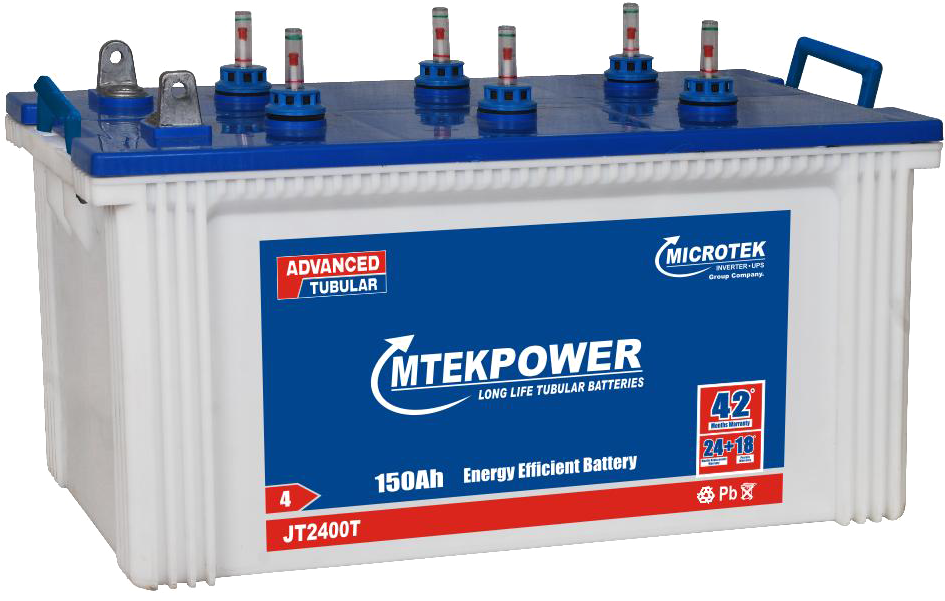
\includegraphics[width=10.86cm,height=6.23cm]{./images/image8.png}
        \caption{Battery}

	\end{figure}

	
          
	 \subsection{Jumper Cable} Jumper wires are simply wires that have connector pins at each end, allowing them to be used to connect two points to each other without soldering. Jumper wires are typically used with breadboards and other prototyping tools in order to make it easy to change a circuit as needed. Fairly simple. In fact, it doesn’t get much more basic than jumper wires.
	
	\begin{figure}[H]
	\centering
	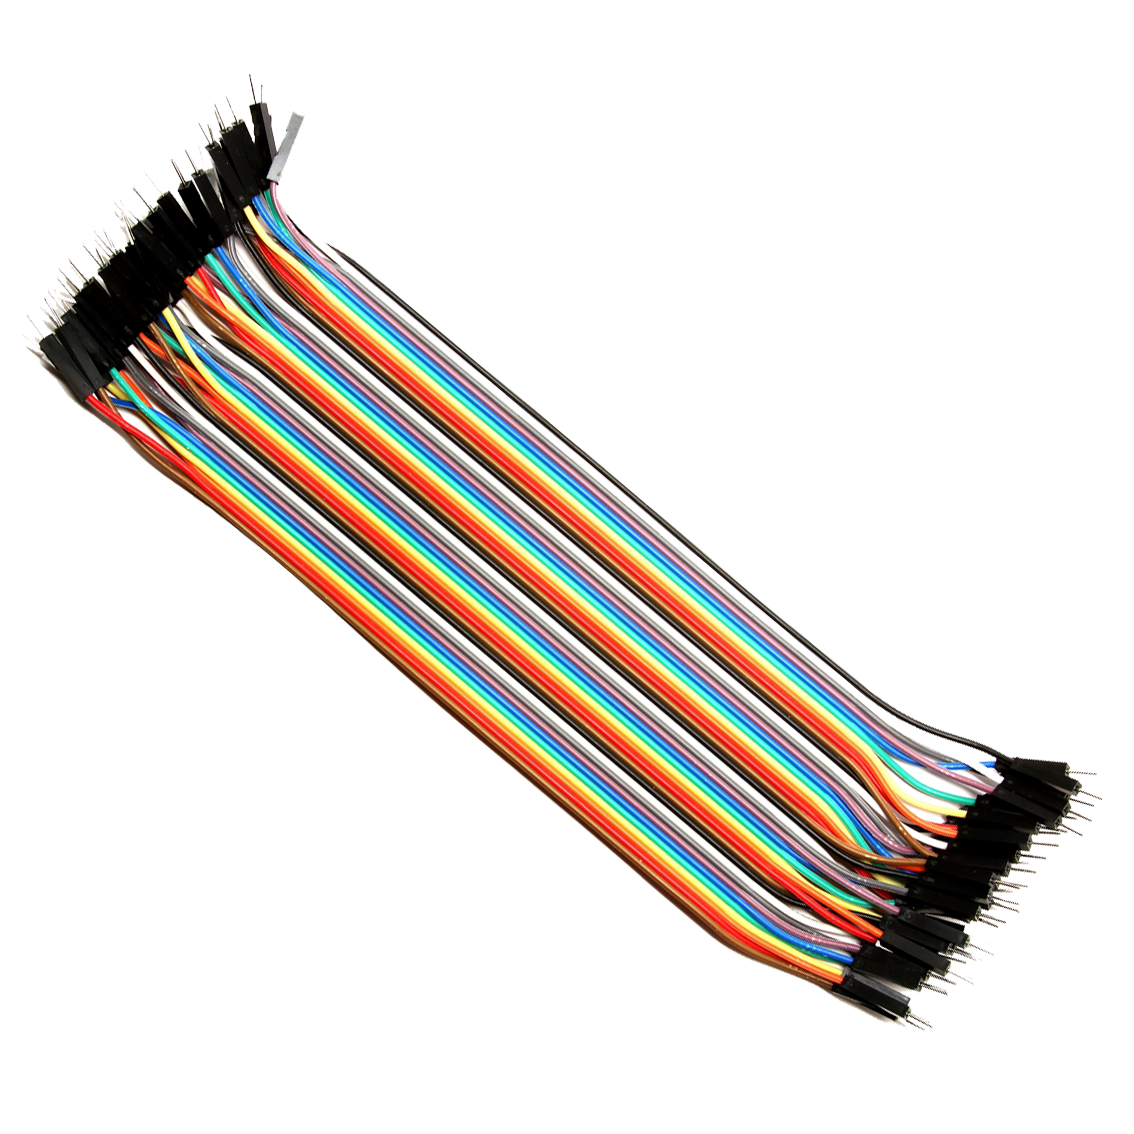
\includegraphics[width=10.86cm,height=6.23cm]{./images/image9.png}
        \caption{Jumper Cable}

	\end{figure}
   
 \subsection{Power Supply} A DC 5V power supply works by converting an input voltage, typically AC (alternating current), to a regulated 5V DC (direct current) output. Several components and techniques are involved in the process of converting the input voltage to a 5V DC output, as explained below:


Lorem Ipsum is simply dummy text of the printing and typesetting industry. Lorem Ipsum has been the industry's standard dummy text ever since the 1500s, when an unknown printer took a galley of type and scrambled it to make a type specimen book. It has survived not only five centuries, but also the leap into electronic typesetting, remaining essentially unchanged. It was popularised in the 1960s with the release of Letraset sheets containing Lorem Ipsum passages, and more recently with desktop publishing software like Aldus PageMaker including versions of Lorem Ipsum.
	\vspace{3\baselineskip}
    \begin{center}
        \Large Write here with your requirements.
    \end{center}
	\vspace{3\baselineskip}
	
	\begin{figure}[H]
	\centering
	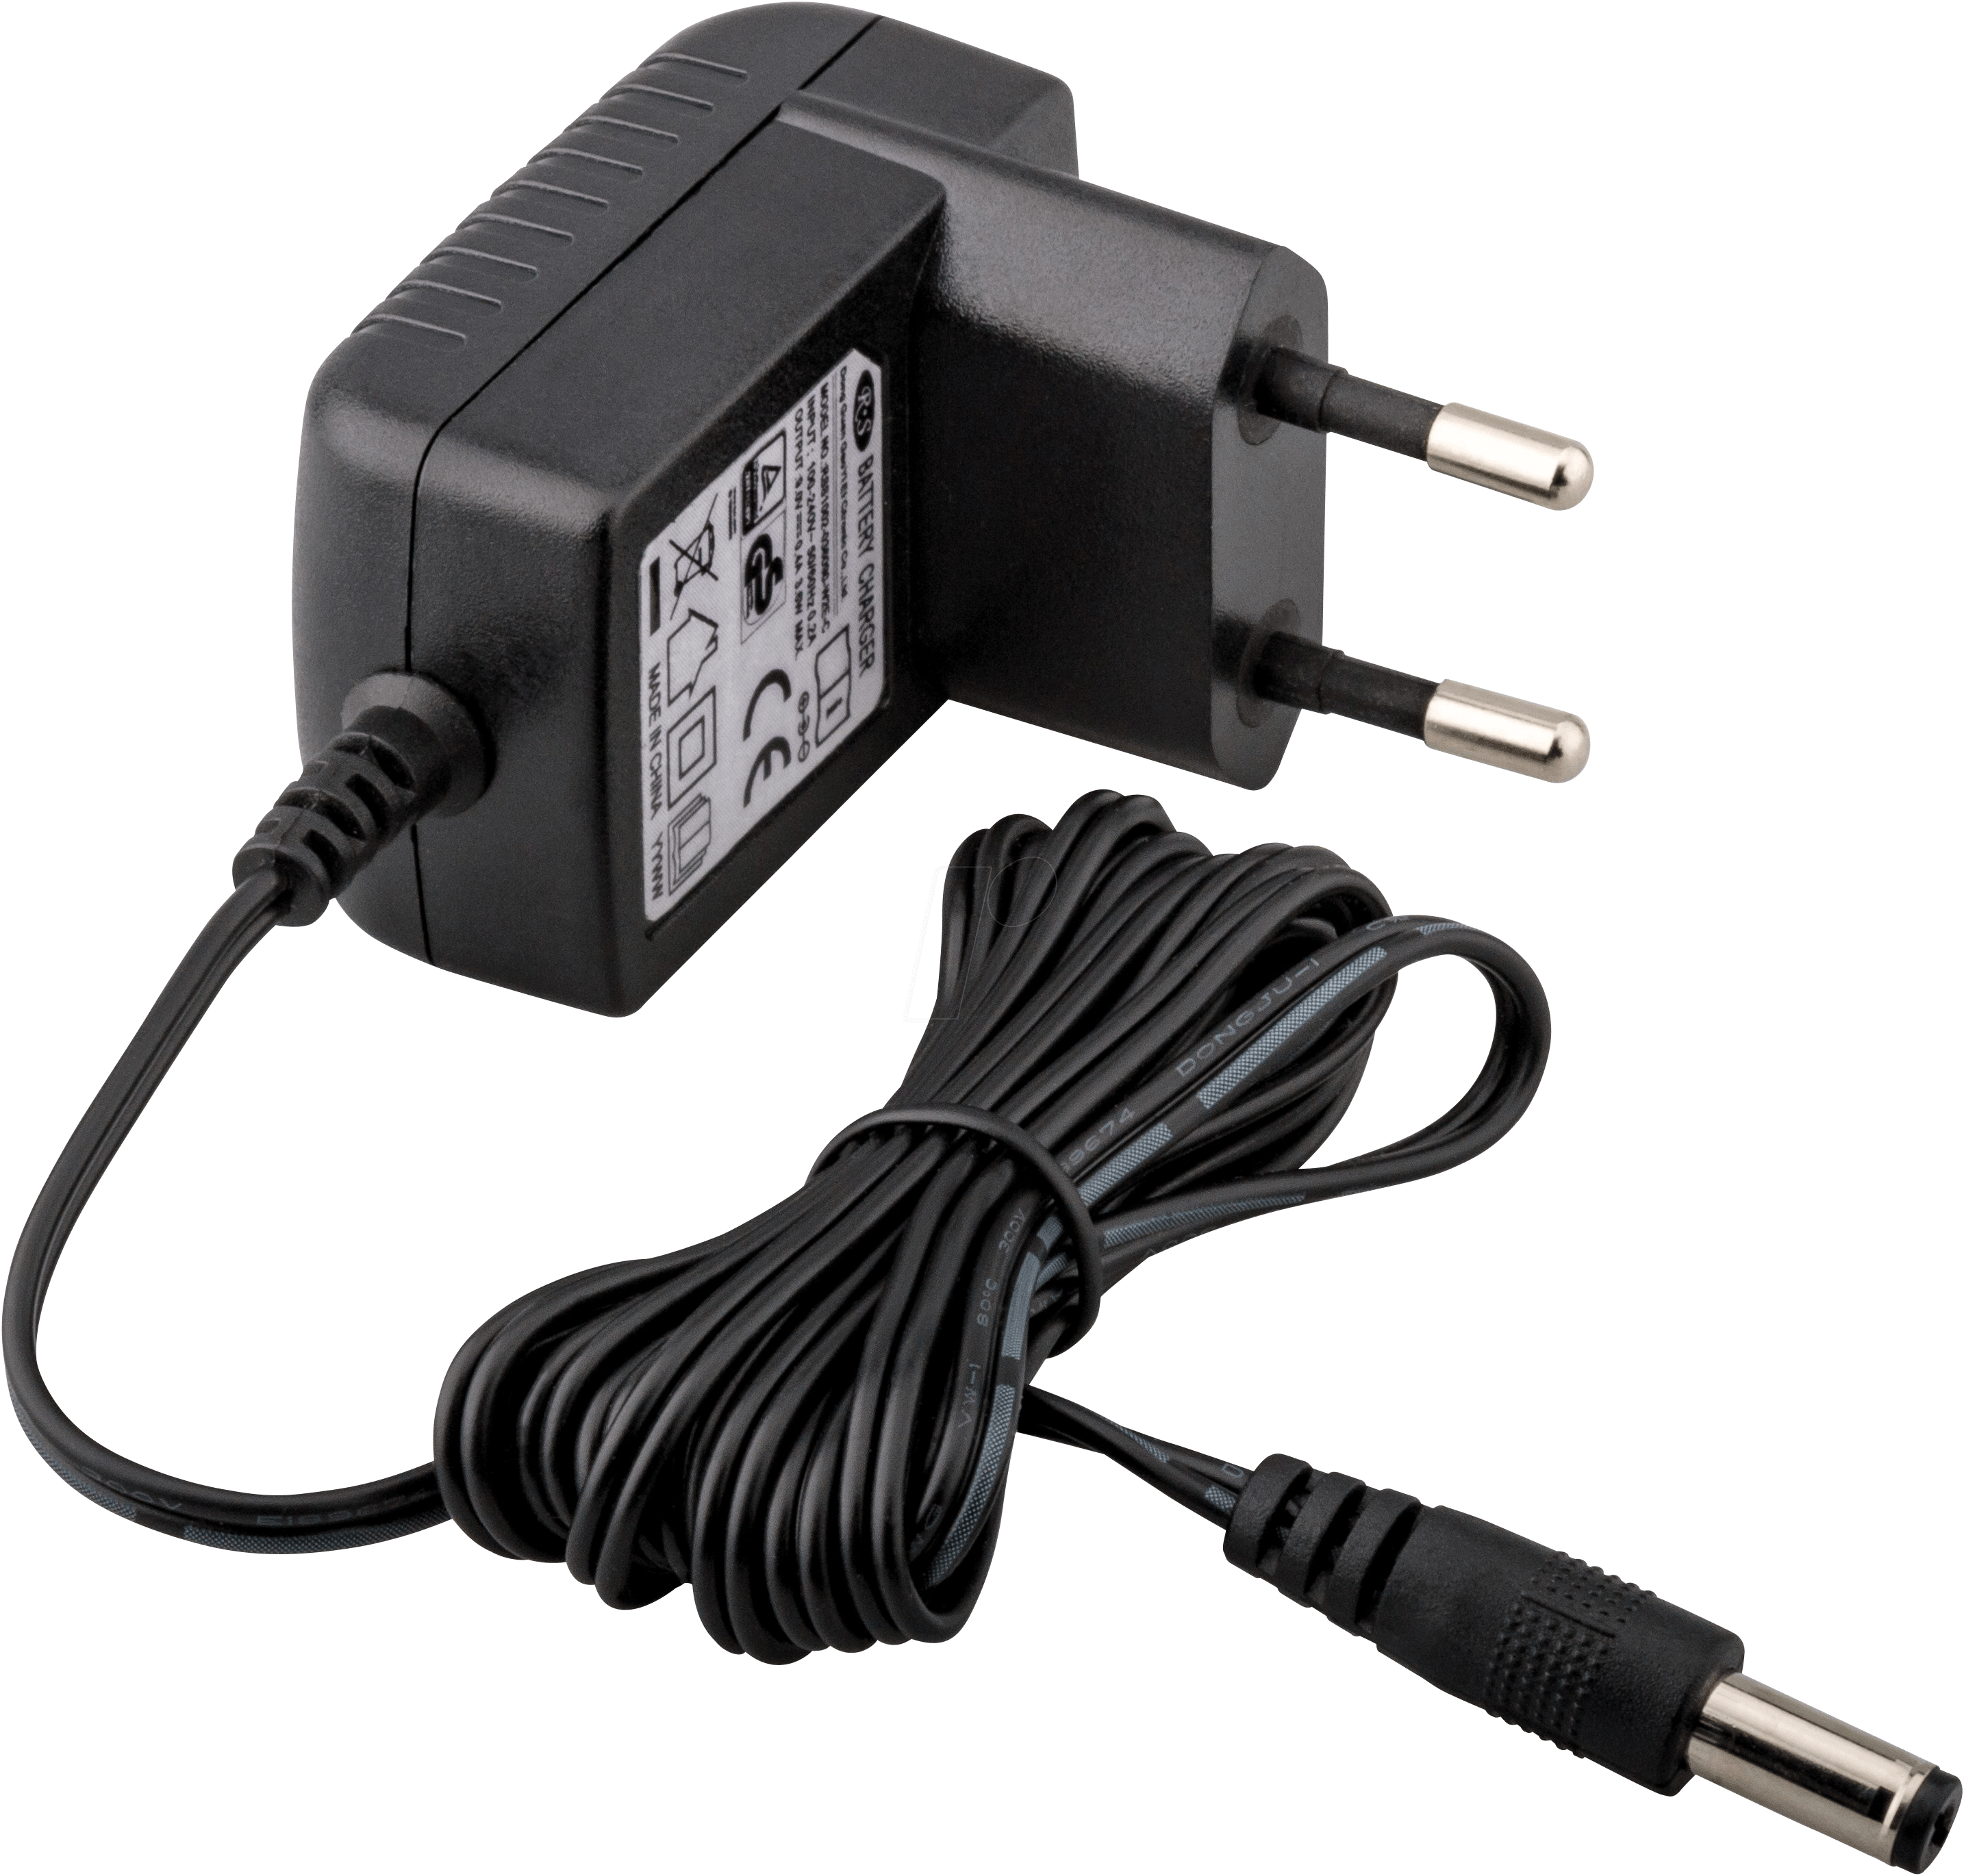
\includegraphics[width=10.86cm,height=6.23cm]{./images/image10.png}
        \caption{Power Supply}

	\end{figure}


\subsection{Software : \textbf{Arduino IDE}}
\vspace{1\baselineskip}
	\begin{figure}[H]
	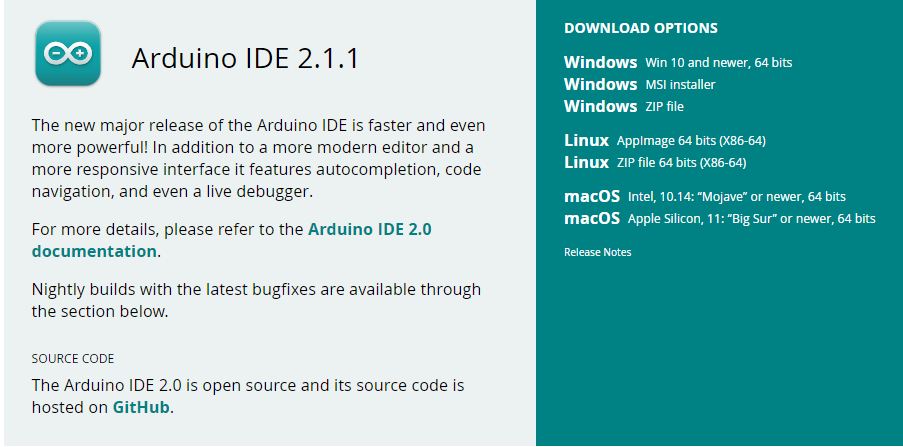
\includegraphics[width=14.33cm,height=7.31cm]{./images/arduino_ide.png}
	\end{figure}
	
	
	The Arduino IDE is an open-source software, which is used to write and upload code to the Arduino boards. The IDE application is suitable for different operating systems such as Windows, Mac OS X, and Linux. It supports the programming languages C and C++. Here, IDE stands for Integrated Development Environment.
	
	The program or code written in the Arduino IDE is often called as sketching. We need to connect the Genuino and Arduino board with the IDE to upload the sketch written in the Arduino IDE software. The sketch is saved with the extension 
	\break
	\textbf{Toolbar Button}
	
	The icons displayed on the toolbar are \textbf{New, Open, Save, Upload,} and \textbf{Verify}.
	
	It is shown below:
	

	
	
	\textbf{Upload}
	
	Lorem Ipsum is simply dummy text of the printing and typesetting industry. Lorem Ipsum has been the industry's standard dummy text ever since the 1500s, when an unknown printer took a galley of type and scrambled it to make a type specimen book. It has survived not only five centuries, but also the leap into electronic typesetting, remaining essentially unchanged. It was popularised in the 1960s with the release of Letraset sheets containing Lorem Ipsum passages, and more recently with desktop publishing software like Aldus PageMaker including versions of Lorem Ipsum.
	\vspace{3\baselineskip}
    \begin{center}
        \Large Write here with your requirements.
    \end{center}
	\vspace{3\baselineskip}
	
	
	
	

\newpage


        \begin{center}
	{\Large\textbf{\section{Code}}}
	\end{center}
	 * Code are started from below for \textbf{Arduino UNO R3}:
        \vspace{2\baselineskip}
        \verbatiminput{code/code.txt}






